\subsection{Measured optimized-baseline and research comparisons}

\label{sec:supplement-results}

Table~\ref{tab:supplement-selector} reports separately timed default SCIC against in-environment static paths. Ratios below one are slowdowns. Eager-relative gains do not imply an improvement over default compilation. The attention native reference is SDPA plus RMSNorm, not materialized attention. Max-autotune ratios use only common numerically admitted samples, whose counts are shown in parentheses.

\begin{table*}[t]

\centering\small

\caption{Executed ridge-plus-compute SCIC. Each ratio is a geometric mean of paired CUDA-event latencies. Direct calls and controlled whole-chain graph replay are separate. $n$ counts process/shape pairs; max-autotune uses common admitted pairs.}

\label{tab:supplement-selector}

\begin{tabular}{@{}lllrrrr@{}}

\toprule

PyTorch & Workload & Timing & $n$ & / native & / default & / max-no-graph ($n$) \\

\midrule

2.5.1 & GEMM & Direct & 126 & 1.225 & 0.890 & 0.839 (116) \\

2.5.1 & Attention & Direct & 54 & 1.045 & 0.830 & 0.831 (54) \\

2.5.1 & GEMM & Graph & 126 & 1.203 & 0.835 & 0.804 (116) \\

2.5.1 & Attention & Graph & 54 & 1.031 & 0.765 & 0.762 (54) \\

2.14.1 & GEMM & Direct & 126 & 1.161 & 0.922 & 0.834 (114) \\

2.14.1 & Attention & Direct & 54 & 0.982 & 0.880 & 0.900 (54) \\

2.14.1 & GEMM & Graph & 126 & 1.359 & 0.866 & 0.897 (114) \\

2.14.1 & Attention & Graph & 54 & 1.090 & 0.745 & 0.745 (54) \\

\bottomrule

\end{tabular}

\end{table*}

\begin{figure*}[t]

\centering

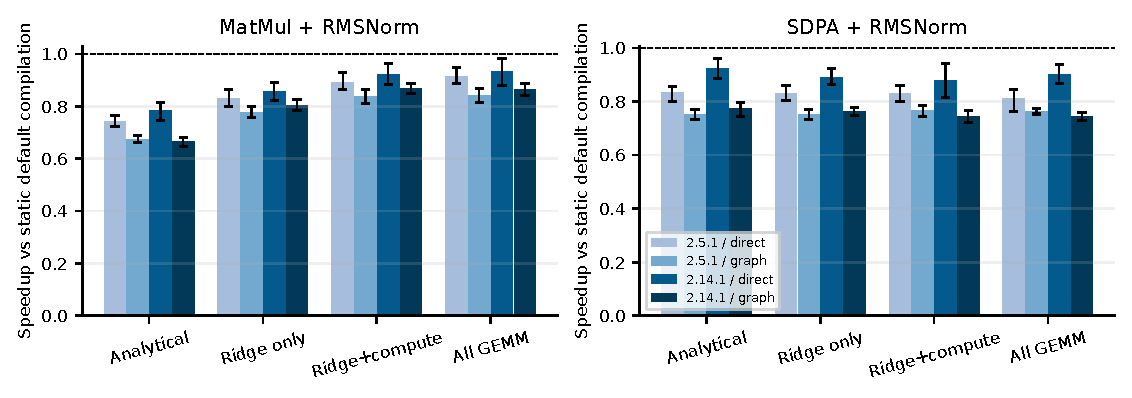
\includegraphics[width=\linewidth]{figures/fig_supplement_selector.pdf}

\caption{Independently timed selection relative to static default compilation, with process-bootstrap intervals. The analytical, ridge-only, default ridge-plus-compute, and all-GEMM scopes share the original $0.5R/2R$ rule. Attention always uses its fixed compiled-SDPA binding.}

\label{fig:supplement-selector}

\end{figure*}

For default-scope GEMM calibration, the following elapsed costs include probe calls and synchronization, after candidate preparation; they exclude compiler preparation and numerical auditing.

PyTorch 2.5.1 / none: 84 probes, median 9.264 ms, p95 146.433 ms.

PyTorch 2.5.1 / manual: 84 probes, median 7.360 ms, p95 145.861 ms.

PyTorch 2.14.1 / none: 84 probes, median 10.272 ms, p95 146.695 ms.

PyTorch 2.14.1 / manual: 84 probes, median 6.953 ms, p95 145.534 ms.

Table~\ref{tab:supplement-research} compares the admitted research artifacts against their matching compiler baselines. These are three process repetitions on one A40 per artifact, not a cross-environment ranking. RedFuser denotes the separately parameterized committed kernel, not successful regeneration.

\begin{table*}[t]

\centering\small

\caption{Complete attention-plus-compiled-RMSNorm research adapters. Default official schedules are used. Unsupported shapes have no timing. Max-no-graph uses the paired count in parentheses.}

\label{tab:supplement-research}

\begin{tabular}{@{}llrrrr@{}}

\toprule

Artifact & Timing & Shapes & Pairs & / default & / max-no-graph ($n$) \\

\midrule

RedFuser committed & Direct & 5 & 15 & 1.237 & 1.340 (15) \\

RedFuser committed & Graph & 5 & 15 & 1.028 & 0.936 (15) \\

Neptune TVM & Direct & 7 & 21 & 0.700 & 0.727 (21) \\

Neptune TVM & Graph & -- & 0 & unsupported & unsupported \\

Neptune Torch & Direct & 5 & 15 & 0.495 & 0.501 (15) \\

Neptune Torch & Graph & 5 & 15 & 0.958 & 0.983 (15) \\

\bottomrule

\end{tabular}

\end{table*}

The Neptune TVM/Triton bridge terminated with SIGSEGV during whole-chain CUDA Graph capture. Those process failures are retained; later captures are explicitly rejected rather than retried. This is an adapter compatibility boundary and does not invalidate its admitted direct calls.

Per-shape timings, process-bootstrap intervals, candidate admission status, available backend traces, and calibration costs remain in the supplementary analysis archive. The measured candidate minimum is limited to admitted executable paths and is not a global schedule optimum.

The official extracted Torch-callable Triton route requires Python integers for its launch configuration; the retained patch converts the TVM integer values without changing their values or schedules. The initial failed series is preserved separately. The admitted Torch-bridge cases exclude multi-kernel decode composition and GQA.

\paragraph{Framework-managed graphs}

The compiler-managed group retains its own direct default baseline. It measures reduce-overhead and max-autotune with the framework's internal graphs and ordinary, unmarked tensor arguments. Profiler traces contain input-copy kernels. Controlled manual replay instead captures fixed storage, and model parameters have their own framework treatment; these protocols are reported separately.

\begin{table}[t]

\centering\small

\caption{PyTorch 2.14.1 framework-managed graph modes relative to default compilation in the same process. Only admitted pairs enter each ratio.}

\label{tab:compiler-graphs}

\begin{tabular}{@{}llrr@{}}

\toprule

Workload & Mode & Pairs & / default \\

\midrule

attention & max-autotune & 27 & 0.871 \\

attention & reduce-overhead & 27 & 0.906 \\

gemm & max-autotune & 57 & 0.655 \\

gemm & reduce-overhead & 63 & 0.659 \\

\bottomrule

\end{tabular}

\end{table}

\paragraph{FlashAttention-2}

FlashAttention-2 with the same compiled FP32 normalization epilogue is available in the PyTorch 2.5.1 GPU-1 environment. Its admitted coverage is reported explicitly; the CUDA extension is ABI-specific and is not reused in the independent PyTorch 2.14.1 environment.

\begin{table}[t]

\centering\small

\caption{FlashAttention-2 plus compiled RMSNorm relative to the compiled SDPA chain in the same process.}

\label{tab:fa2-supplement}

\begin{tabular}{@{}lrrr@{}}

\toprule

Timing & Shapes & Pairs & / default \\

\midrule

Graph & 9 & 27 & 1.016 \\

Direct & 9 & 18 & 0.651 \\

\bottomrule

\end{tabular}

\end{table}
